\section{Grenzwert von Funktionen}
$\lim_{x \to x_0}f(x) = g$ bedeutet, dass $f(x)$ für $x_0$ gegen $g$ geht.\\
z.B. ist $\lim_{x \to 2} x^2 = 4$, da $x^2$ an der Stelle $2$, genau den Wert $4$ hat.\\
\subsection{Rechnen mit Grenzwerten}
\begin{align*}
    \lim_{x \to x_0}(c \cdot f(x)) & = c \cdot (\lim_{x \to x_0} f(x))
\end{align*}
\begin{align*}
    \lim_{x \to x_0}(f(x) + g(x)) & = \lim_{x \to x_0} f(x) + \lim_{x \to x_0} g(x)
\end{align*}
\begin{align*}
    \lim_{x \to x_0}(f(x) \cdot g(x)) & = (\lim_{x \to x_0} f(x)) \cdot (\lim_{x \to x_0} g(x))
\end{align*}
\begin{align*}
    \lim_{x \to x_0}\frac{f(x)}{g(x)} & = \frac{\lim_{x \to x_0} f(x)}{\lim_{x \to x_0} g(x)}
\end{align*}
\subsection{Gebrochenrationale Funktionen}
\subsubsection{Hebbare Definitionslücke}
Zählerpolynom und Nennerpolynom haben \textbf{beide} eine Nullstelle. Durch kürzen kann die Definitionslücke
aufgehoben werden.
\begin{align*}
    \textcolor{red}{f(x) = \frac{x^2-1}{x-1} = \frac{(x+1)(x-1)}{x-1} = x+1}
\end{align*}
\begin{align*}
    \textcolor{red}{\lim_{x \to 1} f(x) = 2}
\end{align*}
\begin{center}
\begin{tikzpicture}[scale=0.7]
    \begin{axis}[
        axis lines = middle,
        xlabel = $x$,
        ylabel = $y$,
        enlargelimits,
        xmin = -2, xmax = 4,
        ymin = -2, ymax = 4]
        \addplot[domain = -2:4,
        samples = 200,
        smooth,
        thick,
        blue] {(x^2)-1)/(x-1)}; 
        \addplot[only marks, mark=*, mark options={scale=1.5, fill=white}] coordinates {(1,2)};
    \end{axis}
\end{tikzpicture}
\end{center}
\subsubsection{Polstelle}
Wenn \textbf{nur} das Nennerpolynom eine Nullstelle (nach Kürzen) hat, dann hat die Funktion eine Polstelle.
\begin{center}
    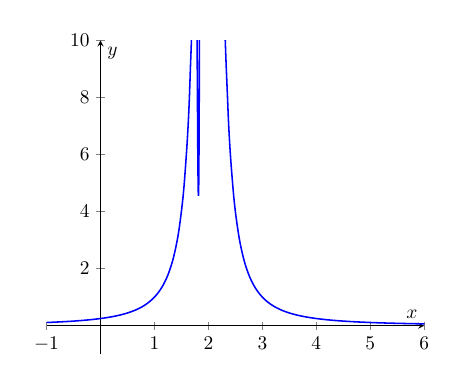
\begin{tikzpicture}[scale=0.7]
        \begin{axis}[
            axis lines = middle,
            xlabel = $x$,
            ylabel = $y$,
            xmin = -1, xmax = 6,
            ymin = -1, ymax = 10]
            \addplot[domain = -10:10,
            samples = 200,
            smooth,
            thick,
            blue] {1/((x-2)^2)};
        \end{axis}
    \end{tikzpicture}
\end{center}
\subsection{Grenzwert von Funktionen in $\infty$}
Der Grenzwert $g$ einer Funktion $f$ für $x \to \infty$ bezeichnet den Wert, der die Funktion annimmt, 
wenn $x$ gegen unendlich geht.
\subsection{Stetigkeit von Funktionen}
Eine Funktion $f(x)$ heisst \textbf{stetig} an der Stelle $x_0$, wenn der Grenzwert von 
$\lim_{x \to x_0} f(x)$ existiert und $= f(x_0)$ ist. Vereinfacht, eine Funktion ist auf einem Intervall 
$I$ stetig, wenn sich ihr Graph in einem Zug, ohne Absetzen, zeichnen lässt.
\subsubsection{Stetigkeits-Aufgaben}
\begin{enumerate}
    \item Prüfen welche Schritte machen (muss ich noch Ableiten für z.B. Differenzierbarkeit?)
    \item Gleichungen für $f_1(1) = f_2(1)$, $f_2(2) = f_3(2)$... usw. aufstellen.
    \item Nach Unbekannter auflösen.
\end{enumerate}
\subsubsection{Einschachteln von Nullstelle}
Falls eine Funktion $f(x)$ auf einem Intervall $[a, b]$ stetig ist, und $f(a)$ und $f(b)$ verschiedene
Vorzeichen haben, dann hat $f$ in $[a, b]$ mindestens eine Nullstelle.